% How is it implemented?
% What technologies are used?
% General Architecture Overview

\section{Methodology}\label{sec:Methodology}
\subsection{Frontend}
Using a website as the user interface offers the advantages of quick and efficient development, broad accessibility across devices, and extensive support for backend technologies. The frontend is built using a tech stack comprising React as the core framework, NextJS for server-side rendering and routing, TailwindCSS for consistent and efficient styling, and NextUI as the component library.

The website is organized into three main pages: the Weather page provides a quick forecast for the current and upcoming days, the Food Stock page displays a categorized list of food items with their expiration dates and storage locations, and the Todos page presents a simple to-do list for daily tasks (Figure~\ref{fig:website}).

\begin{figure}[H]
\includegraphics[width=0.475\textwidth]{media/weather.png}
\includegraphics[width=0.475\textwidth]{media/food.png}
\includegraphics[width=0.475\textwidth]{media/todo.png}
\caption{Website Pages}
\label{fig:website}
\end{figure}

Before accessing the main features, users must authenticate via a login page that supports both email and password registration as well as Google login. Upon successful authentication, users are directed to the main dashboard, where their personalized data is displayed (Figure~\ref{fig:login}).

\begin{figure}[H]
\centering
\includegraphics[width=0.475\textwidth]{media/login.png}
\caption{Login Screen}
\label{fig:login}
\end{figure}

\subsection{External APIs}
Dynamic background images are retrieved from the Unsplash API and cached on the server side for one hour to maintain a fresh appearance without exceeding the free-tier limit of 50 requests per hour. Weather data, including the current conditions and a 5-day forecast, is sourced from the OpenWeatherMap API. This API offers a user-friendly interface for retrieving essential weather metrics such as temperature, humidity, and atmospheric pressure.

\subsection{Backend}
The website is hosted on Vercel at \url{https://cds-dashboard.vercel.app/}, which provides seamless deployment of NextJS applications stored in a GitHub repository. The application is automatically deployed upon each push to the main branch, making it a convenient solution for managing project updates.

User data, such as food inventory and to-dos, is stored in a Supabase database. Supabase, an open-source alternative to Firebase, supports both cloud and self-hosted deployments. While alternatives like MongoDB or traditional SQL databases exist, Supabase offers built-in authentication and API features that reduce setup complexity.

For local deployment, the Supabase Docker image can be pulled and run on any Docker-compatible device, such as a Raspberry Pi. Supabase provides a web interface for database management, and schemas can be imported and configured automatically via CSV files (Figure~\ref{fig:schema}).

\begin{figure}[H]
\centering
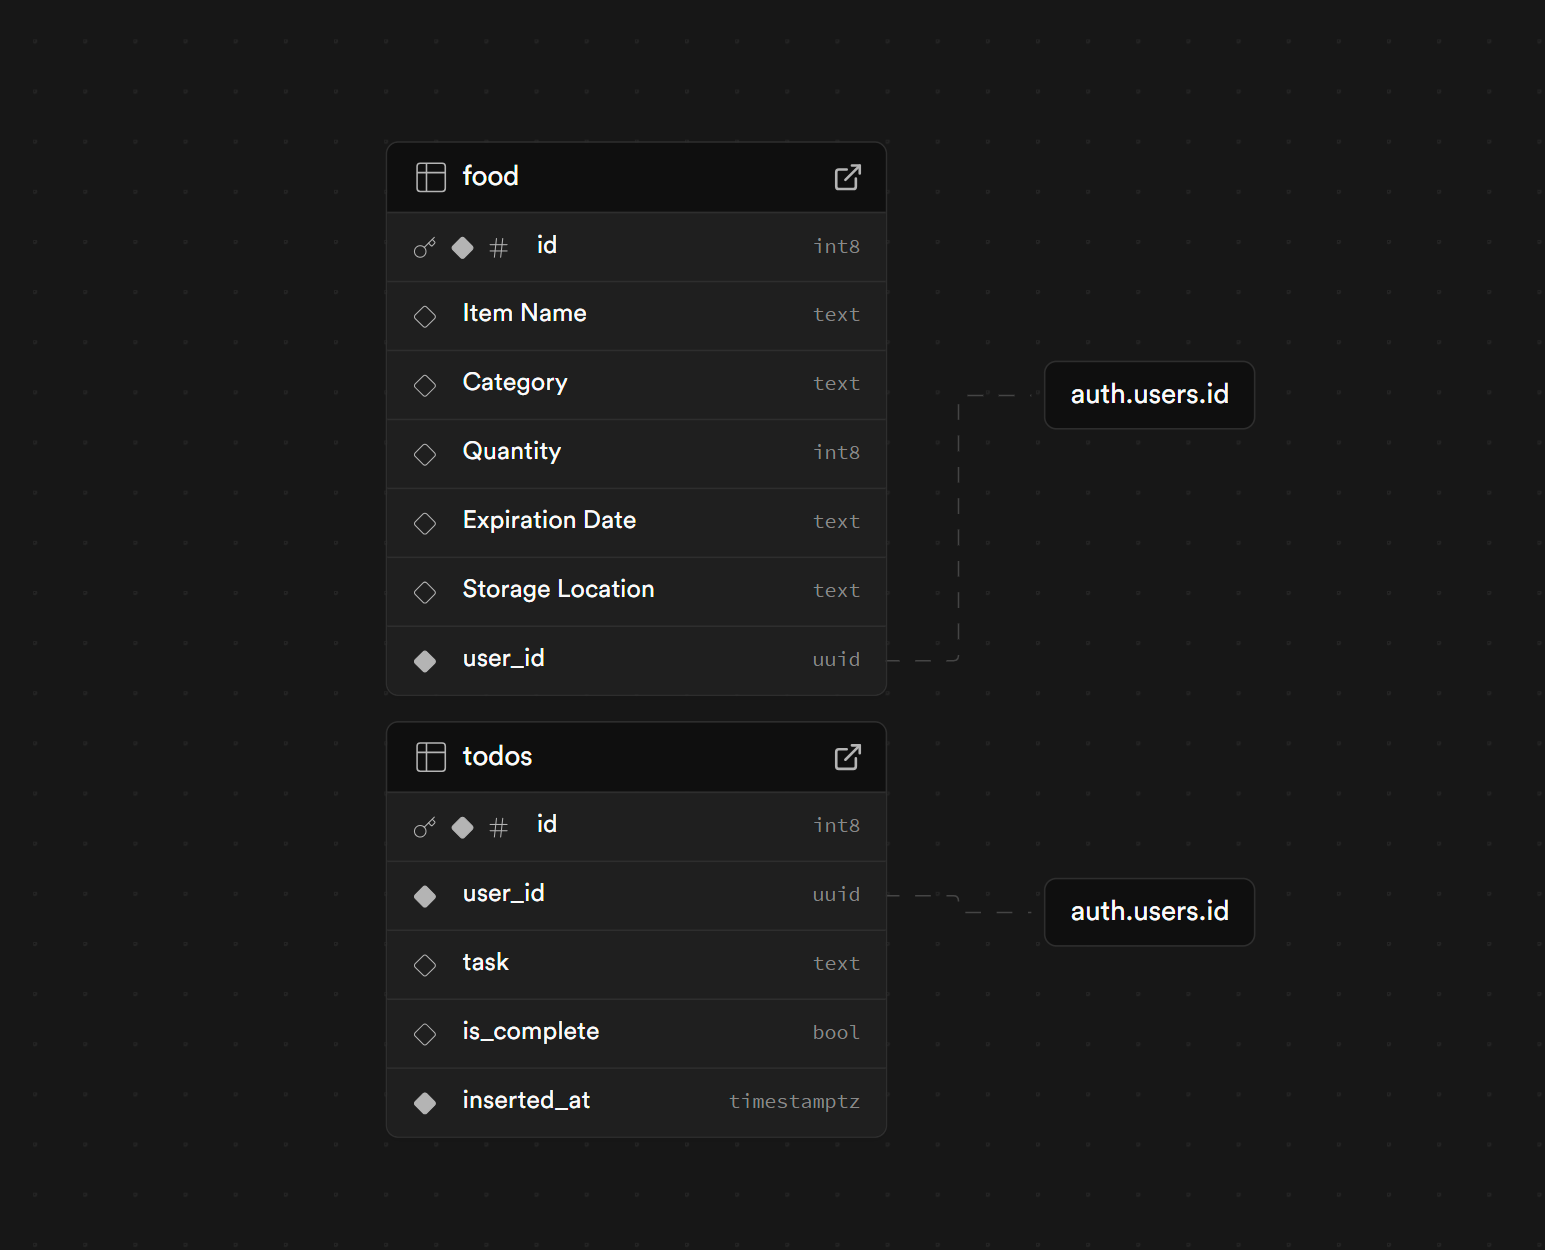
\includegraphics[width=0.475\textwidth]{media/database.png}
\caption{Database Schema}
\label{fig:schema}
\end{figure}

\subsection{Tunneling}
Since the Raspberry Pi is only accessible within the local network, port forwarding could be used, though it requires a static IP address, extensive configuration, and presents security risks
~\cite{wang_port_2024}
. A more secure solution is to use a tunneling service like ngrok, which establishes a secure external tunnel to the Raspberry Pi
~\cite{ngrok_documentation}
. Implementing ngrok involves installing the package on the Raspberry Pi, logging into an ngrok account, and running the command \texttt{ngrok http 3000}. The frontend and Google Cloud configuration URLs need to be updated to reflect the ngrok-provided URL to enable remote access.
